\chapter{Reinforcement learning}


\section{Definitions}

\Acl{rl} (\acs{rl}) methods aim to maximize future reward by mapping the possible states of an environment into actions.

\begin{description}
    \item[Optimal decision making] \marginnote{Optimal decision making}
        Aims to maximize rewards and minimize punishments.

        \begin{remark}
            This is a difficult task as the outcome might be delayed or depend on a series of actions.
            
            \begin{descriptionlist}
                \item[Credit assignment problem]
                    Determine how the various factors involved in making a decision contributed to the success or failure of it.
            \end{descriptionlist}
        \end{remark}
\end{description}

\begin{remark}
    Multiple competing sub-systems contribute to learning and controlling behavior in animals.

    \indenttbox
    \begin{example}[Freud's theory of the mind structure]
        The mind is composed of three structures:
        \begin{descriptionlist}
            \item[Ego]
                Mainly works at the conscious level.
                Rational part of the mind that mediates \textit{id} impulses and \textit{superego} inhibitions.

            \item[Superego] 
                Mainly works at the preconscious level.
                Includes one's ideals and morals. Strives for perfection.

            \item[Id] 
                Mainly works at the unconscious level.
                Irrational part of the mind based on basic impulses that seek immediate gratification.
        \end{descriptionlist}
    \end{example}
\end{remark}


\subsection{Learning}

\begin{description}
    \item[Learning] \marginnote{Learning}
        Lasting change in response or behavior originated from experience.

    \item[Non-associative learning] \marginnote{Non-associative learning}
        Change in response or behavior caused by learning the properties of a single stimulus.
        It can result in:
        \begin{descriptionlist}
            \item[Habituation] 
                A decrease in response to a stimulus that is presented repeatedly.
                \begin{example}
                    The first explosion of a firework causes a strong response but the responses to the following ones are much weaker.
                \end{example}

            \item[Sensitization] 
                An increase in response to a stimulus that is presented repeatedly.
                \begin{example}
                    When the skin itches, one will start scratching it.
                \end{example}
        \end{descriptionlist}

    \item[Associative learning] \marginnote{Associative learning}
        Change in response or behavior caused by learning an association of two or more stimuli/events.

        \begin{descriptionlist}
            \item[\Acl{rl}] \marginnote{\Acl{rl}}
                Learn an association between a neutral stimulus (something the body considers irrelevant) and 
                a reinforcer (something the body considers relevant).

                \begin{description}
                    \item[Primary reinforcer] \marginnote{Primary reinforcer}
                        Positive or negative stimulus that is biologically relevant and elicits a response.
                        \begin{example}
                            Food, pain, social interactions, \dots
                        \end{example}

                    \item[Secondary reinforcer] \marginnote{Secondary reinforcer}
                        Positive or negative stimulus that became relevant following associative learning.
                        It elicits a response which usually enables a primary reinforcer.
                \end{description}
        \end{descriptionlist}
\end{description}


\subsection{Learning systems}

\begin{description}
    \item[Pavlovian/classical system] \marginnote{Pavlovian system}
        Form of prediction learning.
        Learns to predict biologically relevant stimuli to trigger an appropriate response (stimulus-outcome associations).

    \item[Instrumental system] \marginnote{Instrumental system}
        Form of control learning to learn action-outcome associations.
        It includes:
        \begin{descriptionlist}
            \item[Habitual system] \marginnote{Habitual system}
                Learn to repeat previously successful actions.
            \item[Goal-directed system] \marginnote{Goal-directed system}
                Evaluate actions based on the prior knowledge of their consequences.
        \end{descriptionlist}
\end{description}

\begin{remark}
    Pavlovian and instrumental systems are not independent.
    By predicting which situations are positive, one can act to reach them through its actions.

    \begin{figure}[H]
        \centering
        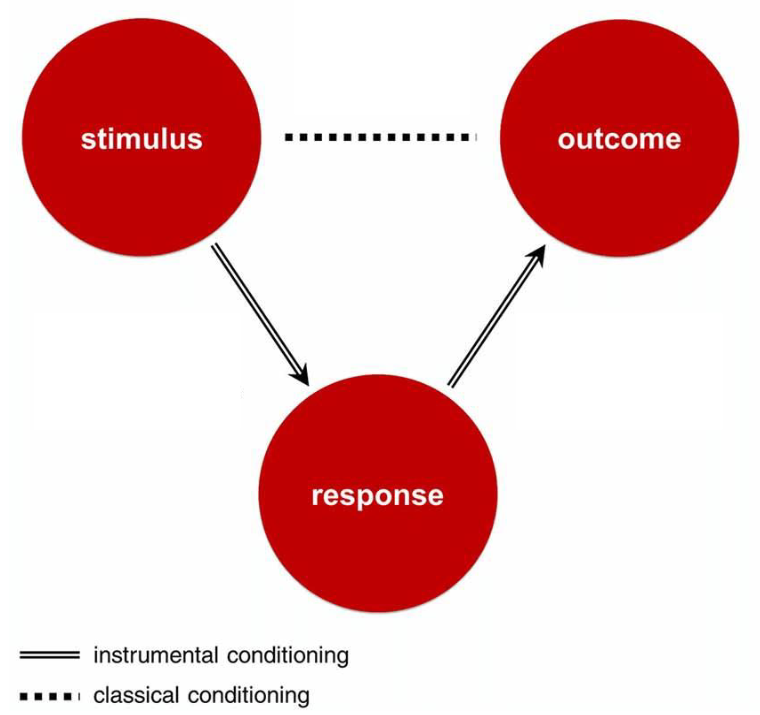
\includegraphics[width=0.35\linewidth]{./img/learning_systems.png}
        \caption{Learning systems relationship}
    \end{figure}
\end{remark}



\section{Learning at the neuronal level}

\begin{description}
    \item[Hebbian plasticity] \marginnote{Hebbian plasticity}
        Learning and experience change the connections of a neural system.

    \item[Short-term change] \marginnote{Short-term neuronal change}
        Functional physiological change that modifies the effectiveness of existing synaptic connections (i.e. amount of neurotransmitters).
        Lasts from seconds up to hours.

    \item[Long-term change] \marginnote{Long-term neuronal change}
        Structural change that leads to anatomical alterations such as pruning or growth of synapses.
        Lasts days and can cause further short-term changes.
\end{description}

\begin{remark}
    Neuronal changes follow a "use it or lose it" policy:
    only useful changes will last.
\end{remark}

\begin{casestudy}[Phantom limb pain]
    In amputees, the area of the brain responsible for the missing part of the body is overrun by the neighboring sections.
    In the case of an arm, the area responsible for the face might "conquer" what once was the area of the arm.
\end{casestudy}



\section{Dopamine}

\begin{description}
    \item[Synaptic plasticity]
        Change the synaptic efficacy by changing the amount of:
        \begin{descriptionlist}
            \item[Neurotransmitters] Directly provoke excitatory or inhibitory effects at postsynaptic neurons.
            \item[Neuromodulators] Neurotransmitters with additional effects.
        \end{descriptionlist}
\end{description}


\begin{description}
    \item[Dopamine] \marginnote{Dopamine}
        Neuromodulator responsible for processes such as motivation, learning, decision-making, addiction, Parkinson's disease, Huntington's disease, \dots.

    \item[Dopaminergic pathways] \marginnote{Dopaminergic pathways}
        \begin{description}
            \item[Nigrostriatal pathway] 
                Originates in the substantia nigra pars compacta (SNc)
                and primarily projects to the caudate-putemen.
                
                \begin{minipage}{0.6\linewidth}
                    \begin{description}
                        \item[Basal ganglia motor loop]
                            Collection of subcortical nuclei responsible for motor control and reinforcement learning.
                            
                            The direct pathway initiates movement while the indirect pathway inhibits it.

                            The SNc projects into the striatum and is responsible for releasing dopamine that activates the direct pathway.
                            The striatum can be seen as the component that uses the reward to influence an action.
                    \end{description}
                \end{minipage}
                \begin{minipage}{0.35\linewidth}
                    \centering
                    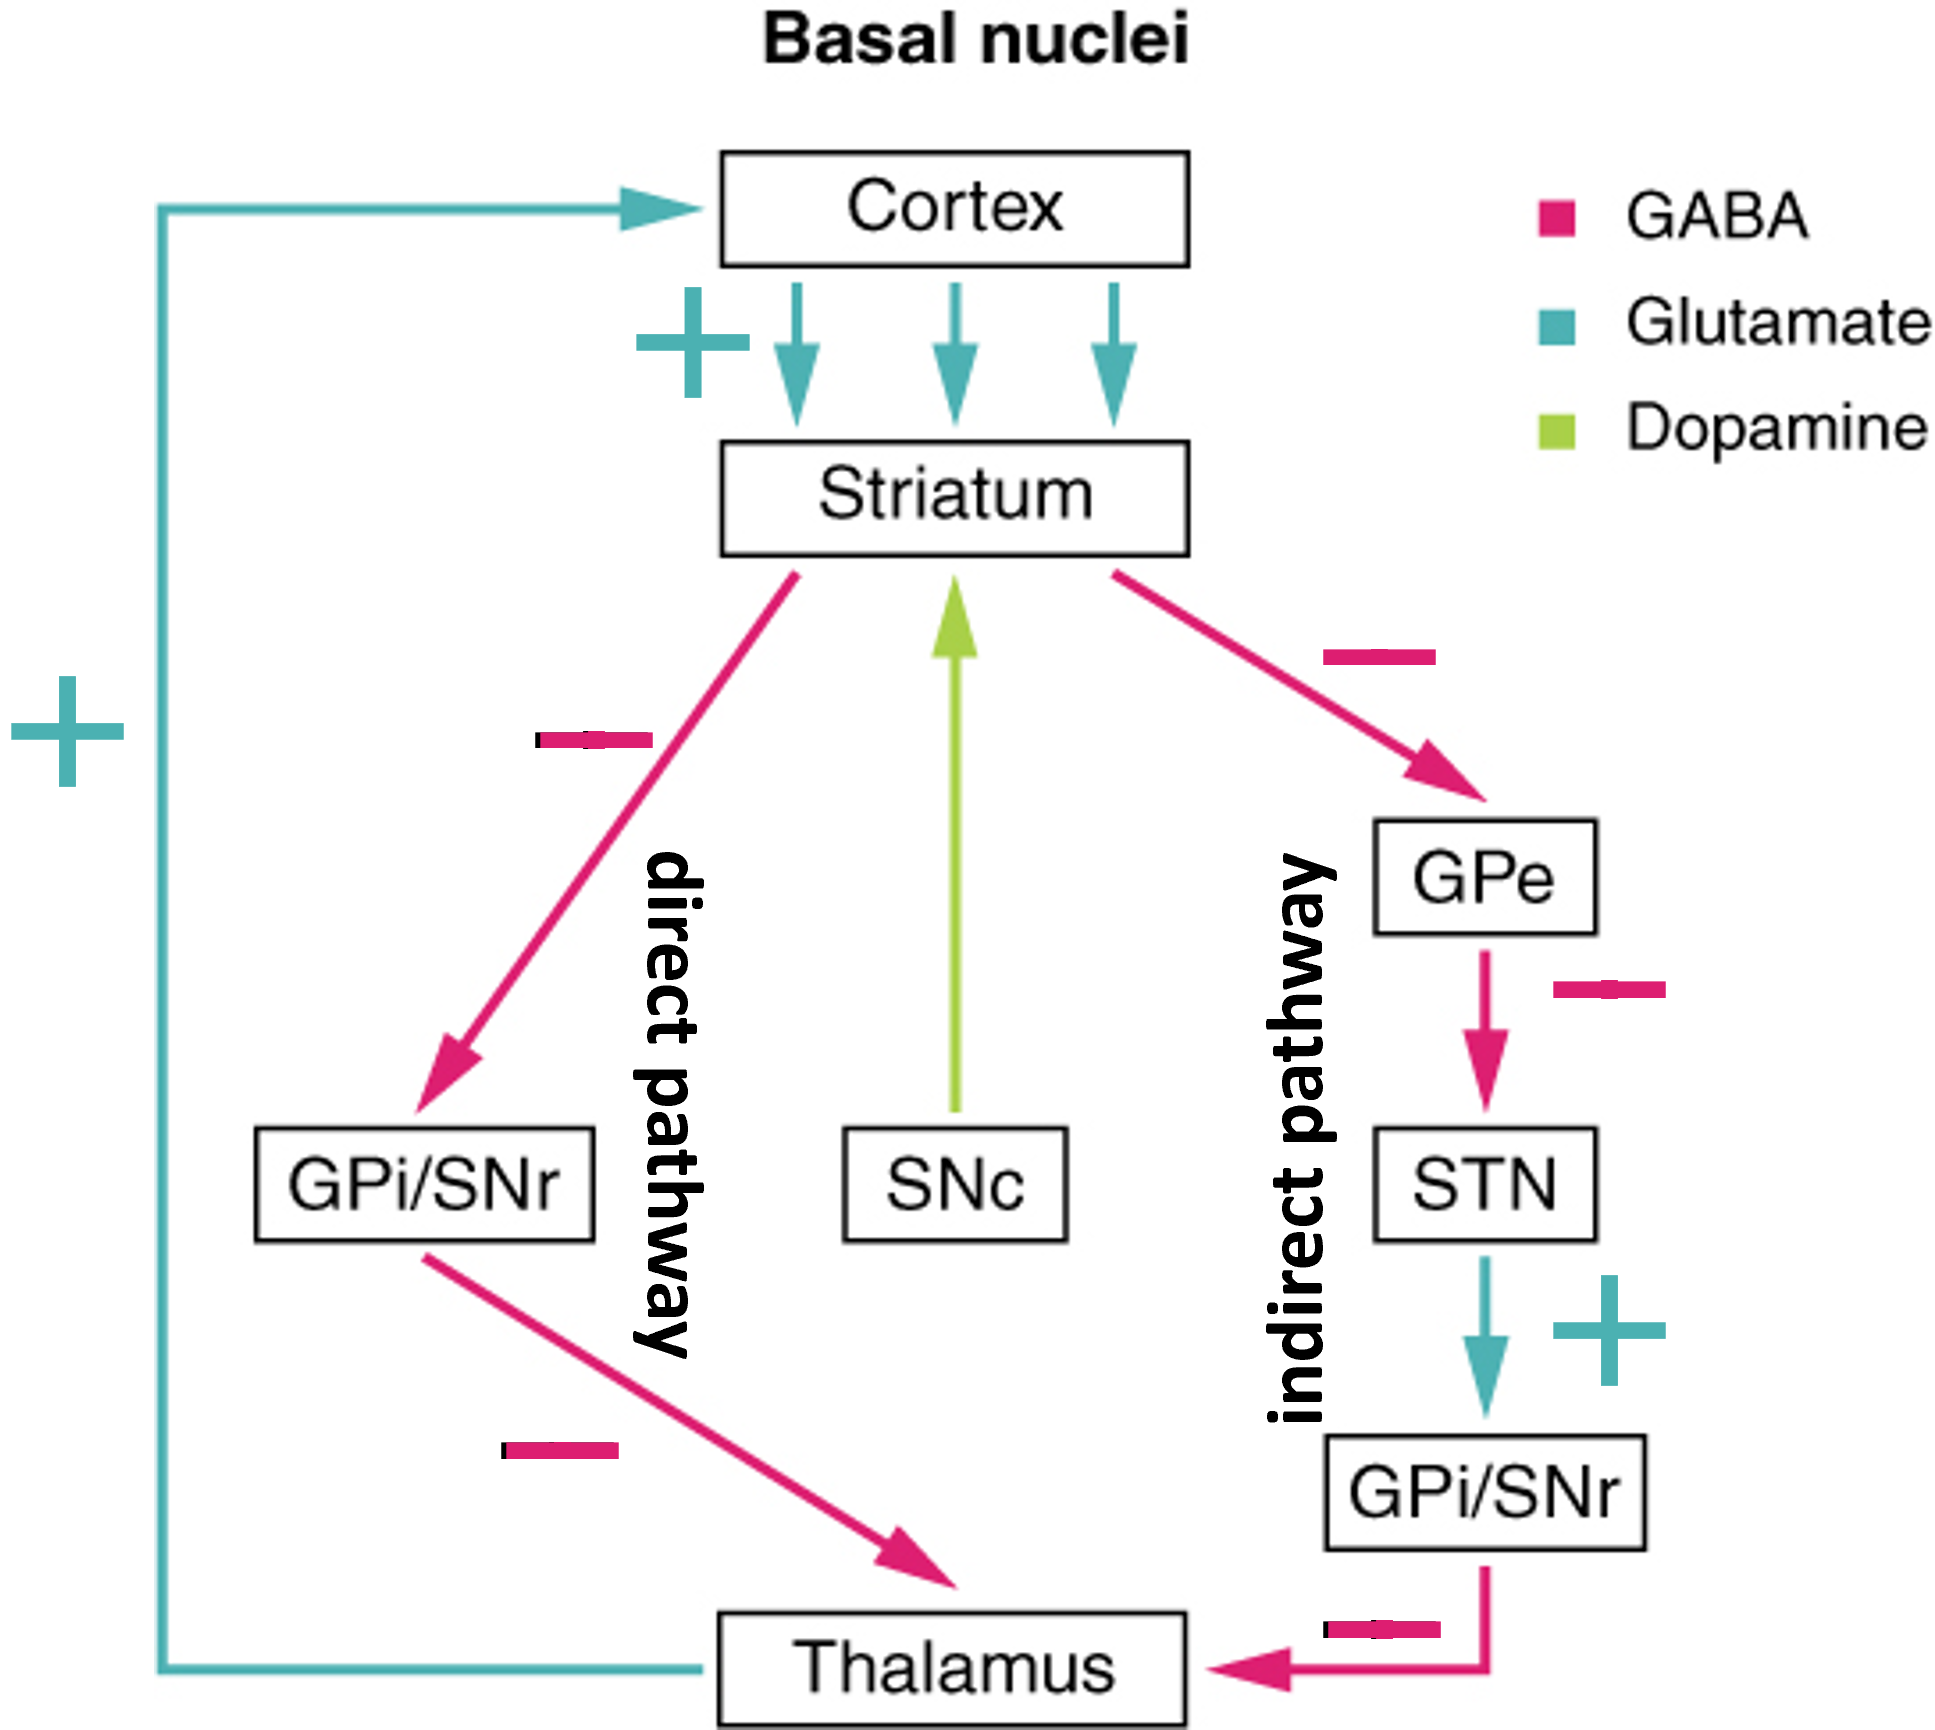
\includegraphics[width=\linewidth]{./img/basal_ganglia_motor.png}
                \end{minipage}

            \item[Meso-limbic pathway] 
                Originates in the VTA and projects to the nucleus accumbens, septum, amygdala and hippocampus.

            \item[Meso-cortical pathway] 
                Originates in the VTA and projects to the medial prefrontal, cingulate, orbitofrontal and perirhinal cortex.
        \end{description}

        \begin{figure}[H]
            \centering
            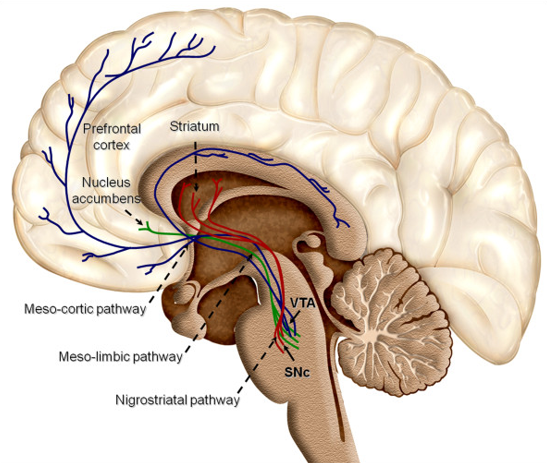
\includegraphics[width=0.3\linewidth]{./img/dopaminergic_pathways.png}
            \caption{Dopaminergic pathways}
        \end{figure}
\end{description}